\documentclass[a4paper,10pt]{article}
\usepackage[english]{babel}
\usepackage[utf8]{inputenc}
\usepackage[toc,page]{appendix}
\usepackage{graphicx}
\usepackage{multirow}
\usepackage{array}
\usepackage{lscape} %pdflscape

%Includes "References" in the table of contents
\usepackage[nottoc]{tocbibind}
\usepackage{titling}
\usepackage{setspace}


\parskip .8ex

%\setlength{\droptitle}{-10em}
\setlength{\topmargin}{-0.5in} % was -1

\usepackage{fancyheadings}
\usepackage{ifthen}
\usepackage{titlesec}
\setlength{\textheight}{10in} %was 10.2

%Begining of the document
\begin{document}

\title{\textbf{CSCM10: Specification}}
\date{8/05/20}
\author{Andy Gray\\445348}



% Build the title and declaration pages, and pad the document so the text starts on a right hand book page.
% Page numbering is in roman numerals until the first page of an actual chapter which resets numbers 
% starting from 1 at that point. 

%\begin{figure}[t]
%	
\includegraphics[width=8cm]{swansea.png}
%	\centering
%\end{figure}
\maketitle
\begin{center}
\item
\includegraphics[width=9cm]{swansea.png}
\end{center}

\thispagestyle{empty}
\newpage
\pagenumbering{arabic}

\begin{abstract}
	As part of our Masters of Science accreditation, we must complete a research thesis. In has been decided upon to create an educational game centred around Machine Learning (ML), due to the authors desire to gain a deeper understanding of ML and their previous experiences as being a secondary school teacher. We have proposed a game that allows the player to interact with different key ML algorithms and models while providing mediums to help educate and teach the players the understanding of the ML and provide knowledge on how they operate. We will achieve this by creating learning research to accompany the game, as well as links to relevant scientific research to get a deeper understanding. While at the centre of it all, having a fun and engaging game, that uses ML to teach about ML. Through using Python, Pygame and industry-standard accepted libraries and packages, like Tensorflow and Sci-kit Learn. The game will provide key gameplay features that users would expect of games, which will be achieved by using fundamental gamification techniques, to create a fun and engaging game that allows the user to interact directly with the ML models. 
\end{abstract}

\clearpage

\section{Introduction}

\small 
As part of our Masters of Science accreditation, we must complete a research thesis. In has been decided upon to create an educational game centred around Machine Learning (ML), due to the authors desire to gain a deeper understanding of ML and their previous experiences as being a secondary school teacher. 


\subsection{Overview of the Problem}
Machine learning gets perceived as a black box, a form of computer wizardry, where unknown algorithms do some magical unknown thing. Some misconceptions people have about Artificial Intelligence (AI) and ML is that 'AI does not need humans' and that 'AI is dangerous' \cite{quora5misconcepts}. Other misconceptions about AI and ML is that they have both very new and based around a human's brain, but AI and ML is something that has been around for a long time, and it is nowhere near the same, even at a fundamental level. Another big misconception is that AI is smarter than humans and that the ML robots will come and destroy the humans wiping out humanity. However, while AI can be better at performing specific tasks, they are not genetically more intelligent than humans. AI will only do what it gets told to do, nothing more \cite{quora5misconcepts}.

On the other hand, instead of fearing AI and ML, there is a lot of this that it is currently doing to help humankind and make things safer. For example, the RAC, one of the UK's largest motoring organisations, aims to try and detect low-speed car crashes. They do this by developing an onboard crash sensing system that uses advanced machine learning algorithms to detect low-speed collisions and distinguish these events from more common driving events, such as driving over speed bumps or potholes. Independent tests showed the RAC system to be 92\% accurate in detecting test crashes, allowing them to be able to enable rapid response to roadside incidents \cite{matlanintrotoml}.

\subsection{Overview of Proposed Solution}
The overall aim of the proposed solution is to create a fun, educating game about ML. The players will be, at the core of the solution, playing a game that interacts with different ML models. The player(s) will be manipulating the game board and data points to affect the decision boundary, or to figure out where the decision boundary or centre of the cluster is. The solution will get created by using  Pygame and will have many different algorithms in the background, doing the main game mechanics, through using libraries like SKLearn \cite{sklearn_api} and Tensorflow \cite{tensorflow2015-whitepaper}.

\subsection{Aims and Objectives}
The proposed solution aims to create a fully interactive game that users will find fun and engaging, while still providing a level of education to teach the players what the different algorithms are and how they work. From the experience of being a teacher, learning has the most impact when the learner gets able to fully interact with the learning subject and see it work first hand, rather than just being told about it. The aim by creating this educational game is to help inform people what ML is and what it does, aiming to demystify the myths and misconceptions around ML.

\subsection{Structure of the Document}
We will first look into background research. Explaining what machine learning with an introduction to what it is, with going into more detail about the different ML techniques. These include supervised vs unsupervised, classification vs segmentation, data-driven approaches, features and dimensionality. An introduction to the machine learning classifiers proceeds the techniques. The classifiers include logistic regression, decision trees, random forests, SVMs and neural networks. We will also look into the literature of gamification and educational games. We will be looking at their impact, and how they get used, what their purpose is how they are adopted and created. We will then explain our proposed methodology, along with our development intentions for the educational game. Including the proposed tools we plan to use and the project management techniques we intend to implement.

\section{Background Research}
\subsection{Intro to Machine Learning}
ML is aiming to teach computers what to do in situations that come naturally to humans and animals, which is to learn from experience. The ML algorithms use computational methods to learn information directly from data, without relying on a predetermined equation as a model. The algorithms improve their performance as the number of samples available for learning increases \cite{matlanintrotoml}.

ML algorithms are finding natural patterns in data, which generates insight. Therefore, allowing humans to make better decisions and predictions. Although some people are very unaware, they get used every day to make critical decisions in medical diagnosis, stock trading, energy load forecasting, and more \cite{matlanintrotoml}. Even media sites rely on ML to sift through millions of options to give personalised suggestions. For example, song or movie recommendations. Retailers use it to gain insight into their customers' purchasing behaviour \cite{matlanintrotoml}.

\subsubsection{Supervised vs Unsupervised}
Machine learning uses two types of techniques: supervised learning, which trains a model on known input and output data so that it can predict future outputs, and unsupervised learning, which finds hidden patterns or intrinsic structures in input data \cite{geron2019hands}. \\
 \\
\textbf{Supervised:} \\
Supervised machine learning aims to build a model that makes predictions based on evidence in the presence of uncertainty. The supervised learning algorithm takes the insights it has gained, from a known set of input data and known responses to the data (output), also known as labels, and trains a model to generate reasonable predictions for the response to new data \cite{matlanintrotoml, geron2019hands}. 

Supervised learning uses classification and regression techniques to develop predictive models. Classification is a technique that predicts discrete responses. The classification aims to classify the inputted data into different categories\cite{matlanintrotoml}. Some examples of this type of technique are deciding if an email is spam or not, or deciding if a patient has a benign or cancerous tumour. These types of applications include credit scoring, medical imaging and speech recognition.

On the other hand, regression techniques try to predict continuous responses \cite{geron2019hands}. An excellent example of this is to check for changes in the temperature or checking the power demands fluctuations. This kind of applications would get used for trading and forecasting electricity load \cite{matlanintrotoml}. \\
 \\
\textbf{Unsupervised Learning:} \\
Unsupervised learning aims to find hidden patterns or intrinsic structures in the data \cite{geron2019hands}. In the same regards as supervised learning, unsupervised learning aims to gain insights from the data. However, whereas supervised learning has the output labels for the provided dataset, unsupervised does not, it aims to explore the data to find patterns or groupings in the data \cite{matlanintrotoml}.

Examples of applications for clustering include gene sequence analysis, market research, and object recognition \cite{matlanintrotoml}.

\subsubsection{Classification vs Segmentation}
As previously mentioned, the classification technique will have predefined classes with the supervised learning getting used \cite{poole2010artificial}. Whereas, segmentation is about grouping similar things together using unsupervised learning, very similar to the clustering technique. For example, with using image processing as the comparison, segmentation is the process of extracting smaller segments out of one image with the intent of identifying different parts or objects within an image. The results od segmentation is that an image can give the analysis background and foreground separately, whereas classification is identifying if an image forms part of a class. For example, the algorithm will be classifying an image as a cartoon or photo \cite{quorasegclusdiff}. 

\subsubsection{Data-Driven Approaches}
Humans naturally have biases, which means that we can, when training a model, take short cuts to get decisions. This situation might seem reasonable. However, biases should not go challenged, one way to challenge biases it to have a data-driven approach (DDA). 

The DDA required that 10 or 20 different algorithms are tested, with doubling down happening on the algorithms that show insights of being a better performer, speed and robustness. Instead of picking the most common parameters, a grid search of as many different parameters gets done. The output of this aims to remove objectivity and anecdotes \cite{DDA}.
\subsubsection{Features and Dimensionality}

\subsection{Introduction to Machine Learning Classifiers}
\subsubsection{Linear and Logistic Regression}
\textbf{Linear regression} is a model that aims to fit a line of best fit to the data provided. In order to do this, the algorithm chooses the best overall score from the 'Root Mean Square Error' (RMSE). Therefore, in order to train a linear regression model, we need to find the value of $0$ that minimises the RMSE \cite{geron2019hands}. \\
\\
\textbf{Logistic regression} is an algorithm that gets used for classification. Logistic regression gets used to estimate the probability that an instance belongs to a particular class. If the estimated probability is greater than 50%, the model predicts that the instance belongs to that class. If the model has predicted that the instance belongs to that class, also known as the positive class, it gets a '1' label \cite{handson book}. 

\subsubsection{Decision Trees and Random Forests}
\textbf{Decision Trees} (DTs) are a very versatile ML algorithm which can perform both classification and regression, ones that also has multioutput tasks \cite{geron2019hands}. DTs is a form of supervised learning that aims to determine an approximate sine curve with a set of if-then-else decision rules. The deeper the DTs is, the more complex the decision rules are. DTs builds classification or regression models in the form of a tree structure. It breaks down a data set into smaller and smaller subsets while at the same time an associated decision tree is incrementally developed. The final result is a tree with decision nodes and leaf nodes. A decision node has two or more branches. Leaf node represents a classification or decision. The topmost decision node in a tree which corresponds to the best predictor called the root node. Decision trees can handle both categorical and numerical data \cite{mediumtrees}. \\
\\
\textbf{Random Forests} fundamental idea behind them is to combine many decision trees into a single model. Individually, predictions made by decision trees (or humans) may not be accurate but combined, the predictions will be closer to the mark on average \cite{towardsdsrandforest}. Random forest is better than a single decision tree because we can think about it terms of having hundreds of humans make estimates for the max temperature problem.  Pooling everyone's predictions, we can incorporate much more knowledge than from anyone individual \cite{towardsdsrandforest}. 

\subsubsection{SVMs}
Support Vector Machine (SVM) is another powerful and versatile ML model. The model is capable of performing linear or nonlinear classification, regression and even outlier detection. SVM is one of the most popular ML models and are best suited for small to medium-sized datasets. SVM aims to separate the data categories by using a decision boundary, with the largest margin between them. The algorithm is known as the 'large margin classification' \cite{geron2019hands}.

\subsubsection{Neural Networks}
Neural Networks (NN) or also known Artificial Neural Networks (ANN), are at the very core of Deep Learning (DL). An ANN is an ML model inspired by networks of biological neurons found in our brains. However, ANN has become very different from their biological cousins that they took inspiration. ANN is what powers Google's image classifications, Apple's Siri and YouTube's video recommendation, as well as learning to beat the worlds best player at the game called Go, named 'DeepMind's Alpha Go' \cite{geron2019hands}.


\subsection{Summary explaining intent to develop the Edu-game for ML}


\section{Proposed Methodology}
\subsection{Introduction to Proposed Application}
Our main aim is to create an educational game, that aims to teach the main concepts of machine learning. The application will offer multiple game modes like 'claim the screen', 'pin the point on the decision boundary', to name a few. The application will allow the players to interact with the primary ML model to be able to get an understanding of how the application works. Along with giving the user a video explanation and text of how the algorithm works as well as having links to critical scientific papers to gain a better in-depth understanding.  

\subsection{Overview of proposed Critical Features}
\subsubsection{Gameplay}
The intended gameplay will use a turn-based style playthrough. The result of this will be that a play, possibly at random between 1 and 2, will make a move, selecting their location to place their data point, then the second mover, then back to the first mover and so on until the players have made three selections each. 

The scoring will get decided upon based on the game mode and the model that is getting used. For example, for the game mode 'Pin the Data Point on the Decision Boundry', the user who has placed their data point closest to the decision boundary will win three points, the second closet two points, and the third closest data point one point. All the six points, if played well by the player, can be won by the same player. A similar mechanic can get used for 'Where is the Cluster's Centre Point' game mode. In regards to the game mode 'Claim the Screen', the points will be award to the player whom managers to have the most amount of game screen once the decision boundary gets created after all data points have gotten inputted into the game.

An educational aspect will get provided into the game through introduction videos to each model, explaining the model and how they work, what are the mechanics behind them. However, not into too much detail as the main focus will be the game itself but additional, more in-depth, videos and educational resources, like a web page explaining how the algorithm works in more detail. With additional content getting unlocked which will provide code snippets and links to academic papers that introduced these concepts.

\subsubsection{Single vs Multiplayer}
The game will be two players, human versus human. However, bonus rounds could get presented to the player, for example, completing a pop quiz on machine learning to gain extra points. Additional game features could include a 'Domination' style gameplay of equal teams of two vs two or three vs three players introduced. However, we do aim to incorporate a single-player game mode into the application that will be the same mechanic of the player vs player but with player vs AI.


\subsection{Overview of proposed optional features}

\subsubsection{Game Modes}
There are three main game types of design at current. These are 'Claim the Screen', 'Pin the Point on the Decision Boundry', 'Where is the Cluster Centre?' and 'Domination'.\\
 \\
\textbf{Claim the Screen}
\\How 'Claim the Screen' will work is that the players will make three data point entries. The algorithm will then place the decision boundary based on the data points entered by all the players. The player that has claimed the higher proportion of the screen, when the decision boundary gets drawn, wins the level. This game mode can get assigned to all of the models, except the clustering algorithms. To implement different difficulty settings within this game setting the game map can be prepopulated with data points, assigned to each player. However, the player association will not get revealed until the end. Once all moves had been made by the players. \\
 \\
\textbf{Pin the Point on the Decision Boundry}
\\As a play of the old party game pin the tail on the donkey, this game mode will be requiring the player to place data points on the screen. The decision boundary of the model will then appear, and the data point with the lowest SME wins the round, in regards to linear regression for this example. The SME is the value giving to the data point to how far away they are to the decision boundary. \\
 \\
\textbf{Where is the Cluster Centre?}
\\This game mode will get used for playing with the clustering algorithms like GMM and Kmeans. The playing area will get prepopulated, and the player will have to guess where the centre of the cluster will be. \\
 \\
\textbf{Domination}
\\For the game mode 'Domination', the essential mechanics would be the same, but the winner will be decided based on how the team overall has done with the team with the best average score winning the round.

\subsubsection{Human vs AI}
While the initial implementation is aiming for the main gameplay to be player versus player at first be its priority. However, depending on time requirements, there is a desire to have an option for single-player action and playing against the computer, or AI, although the initial implementation might be very basic in the form of the AI just making 'random guesses'. With potentially being developed into something this more a little more strategic, and is affected by the move the player has just taken.

\subsubsection{Unlockables}
During the game, when specific actions have happened. The game will reward the player with rewards. The rewards will come in a variety of forms, some in the more traditional gamification methods like badges. However, the main ones will come in the form of code snippets and publication documentation getting unlocked and presented to the player. \\
 \\
\textbf{Code Snippets}\\
When the plays complete the level, as a reward example code will get presented, allowing the player to see how the algorithm works in practice. Along with additional text to explain step by step what the algorithm is doing. \\
 \\
\textbf{Publication links}\\
The players will also get presented with links and future read articles to academic science papers and publications for further readings, to get a better fundamental of the algorithm and also where to go to get to the next step.

\section{Proposed Mock-up prototype images}
The following screens mockups depict some initial ideas of the game screen. It contains information for the locations of where the players have selected, along with a game map which the players can click in, placing their data points.

\begin{center}
	\item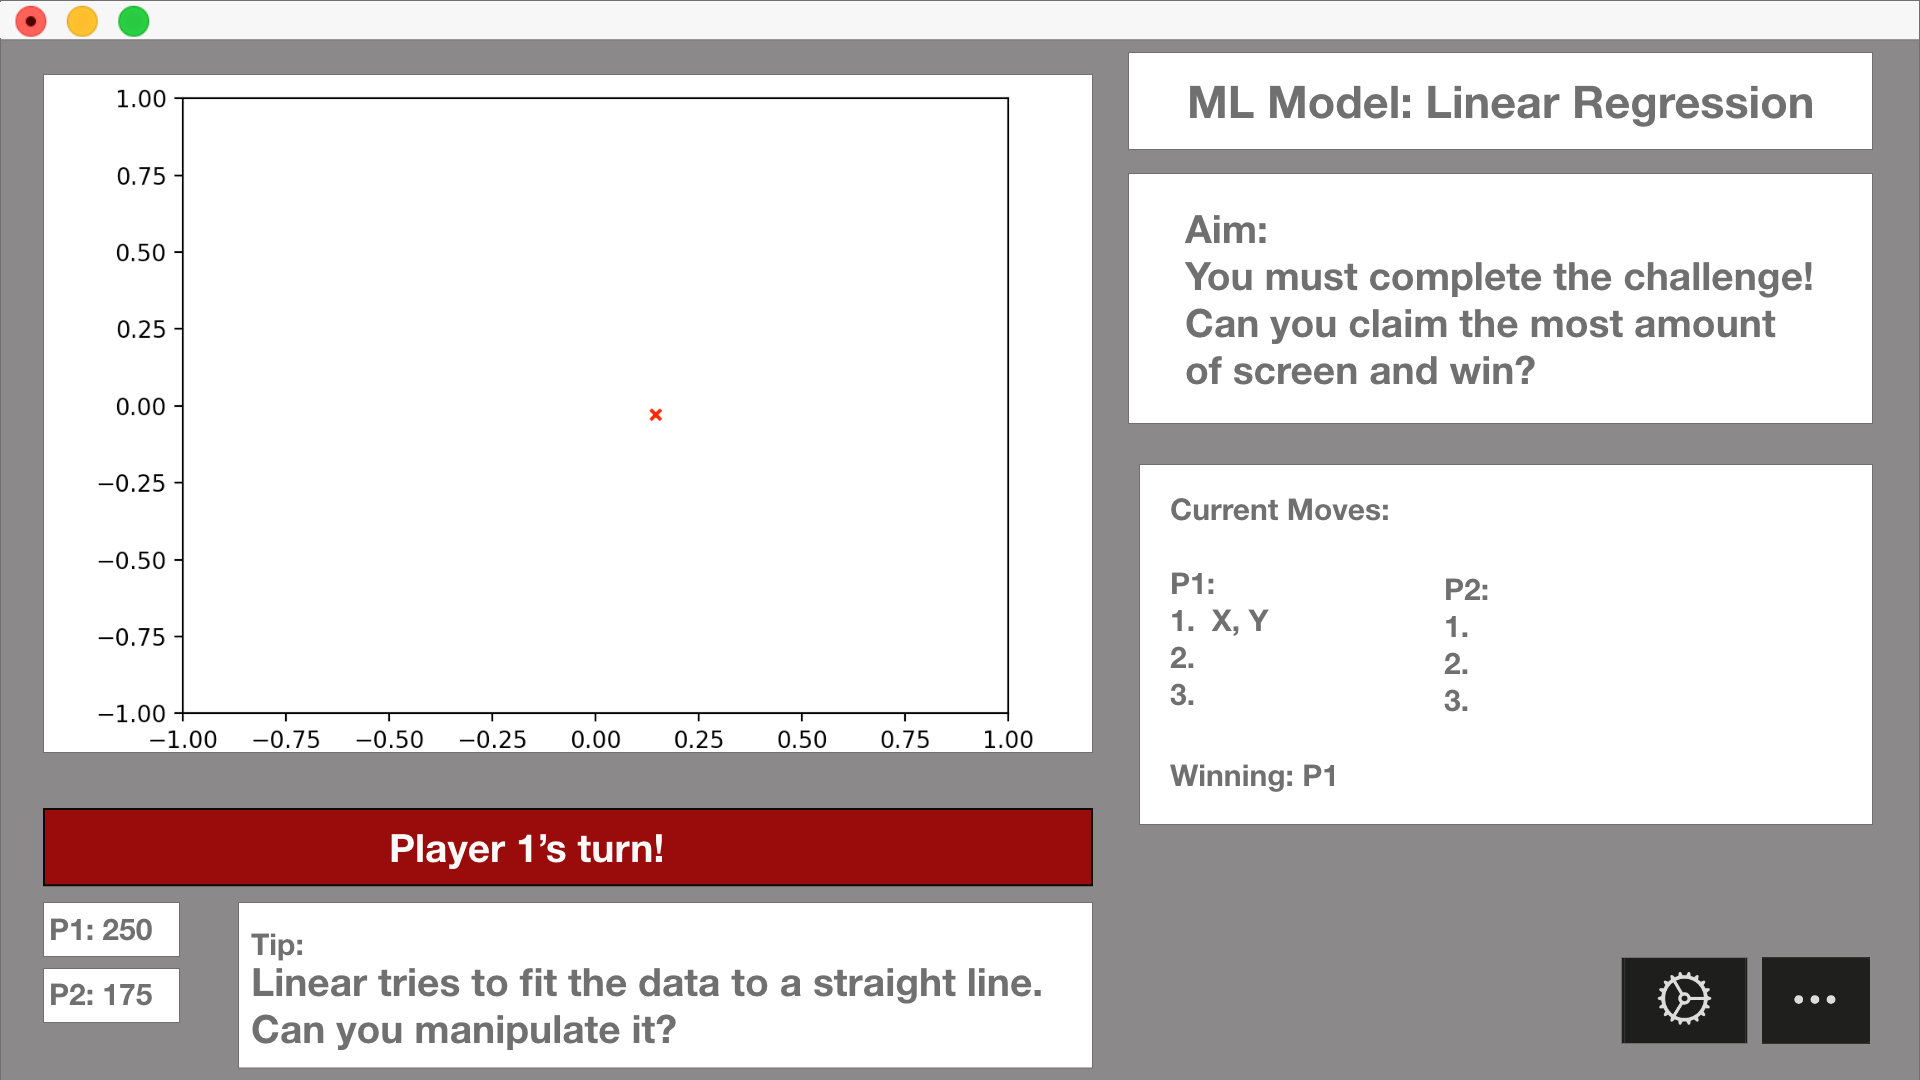
\includegraphics[width=12cm]{Web19201.png}
	\item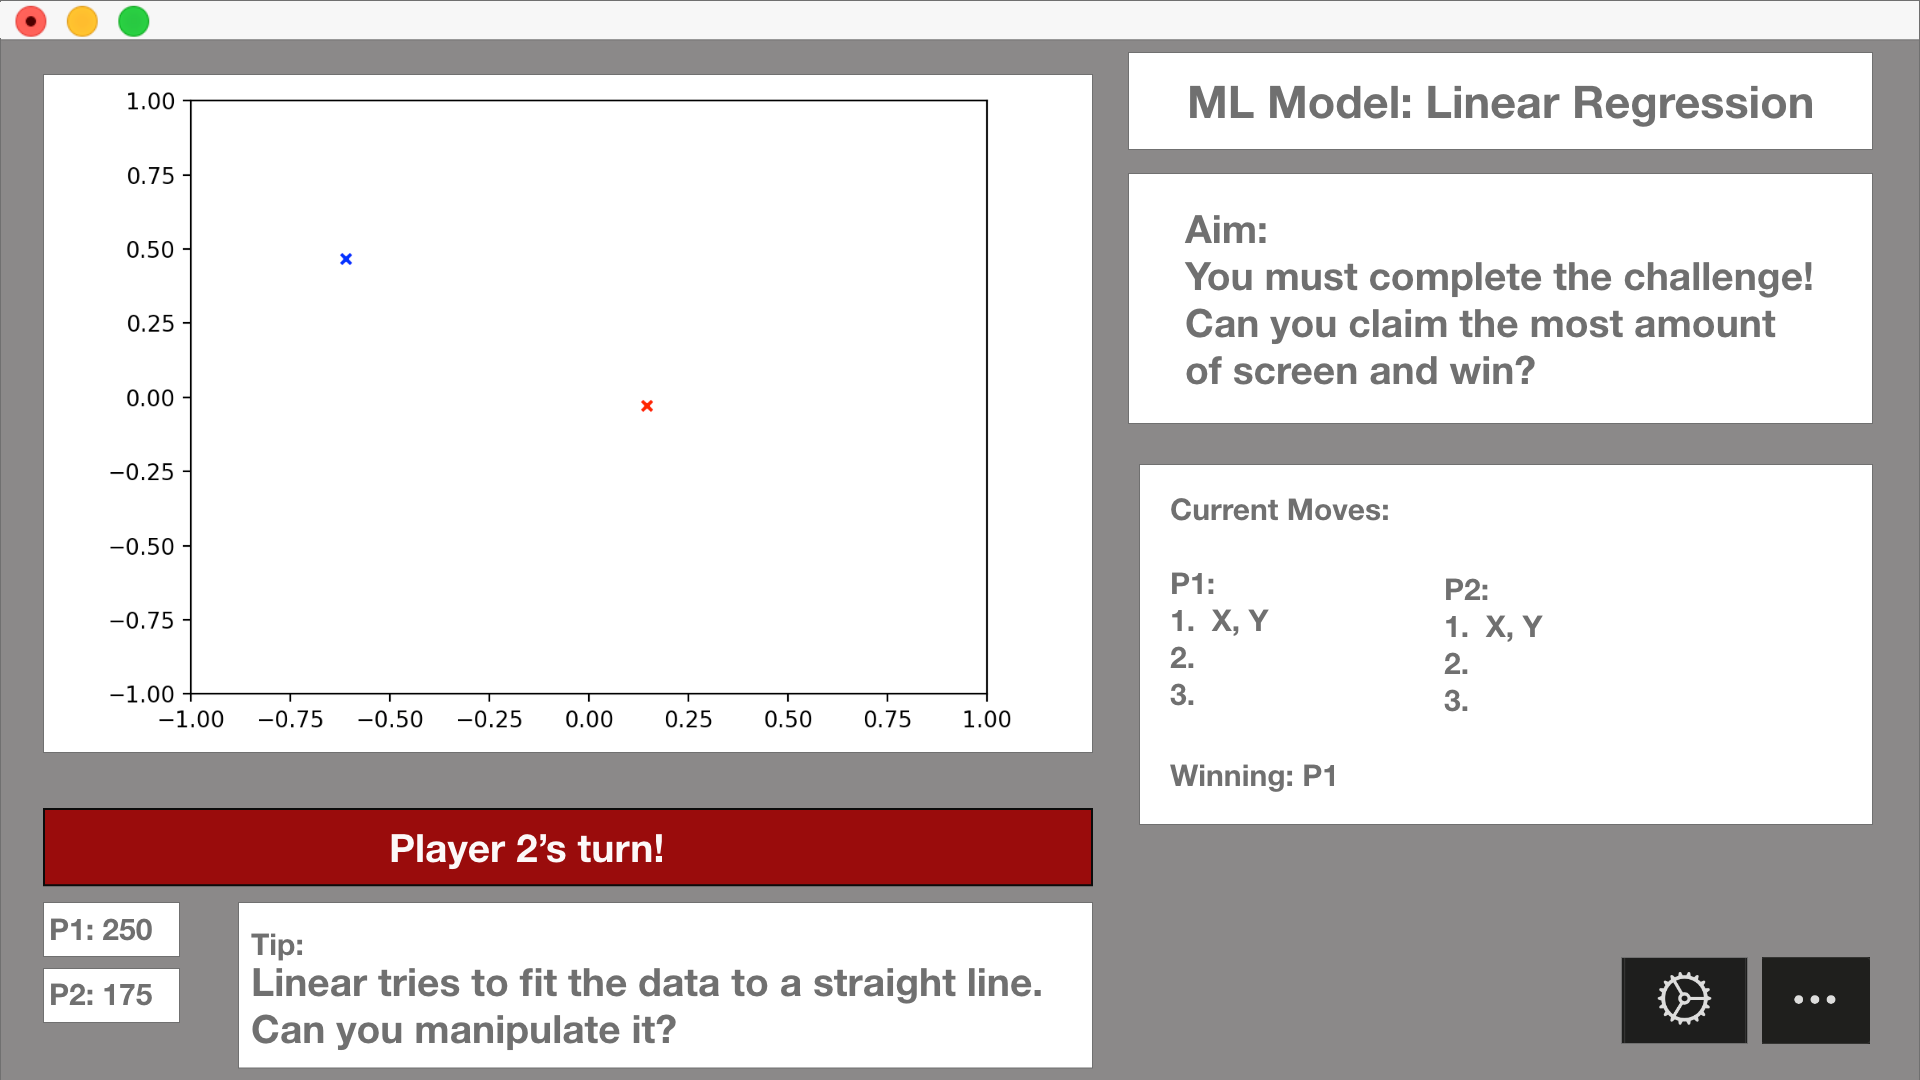
\includegraphics[width=12cm]{Web19202.png}
	\item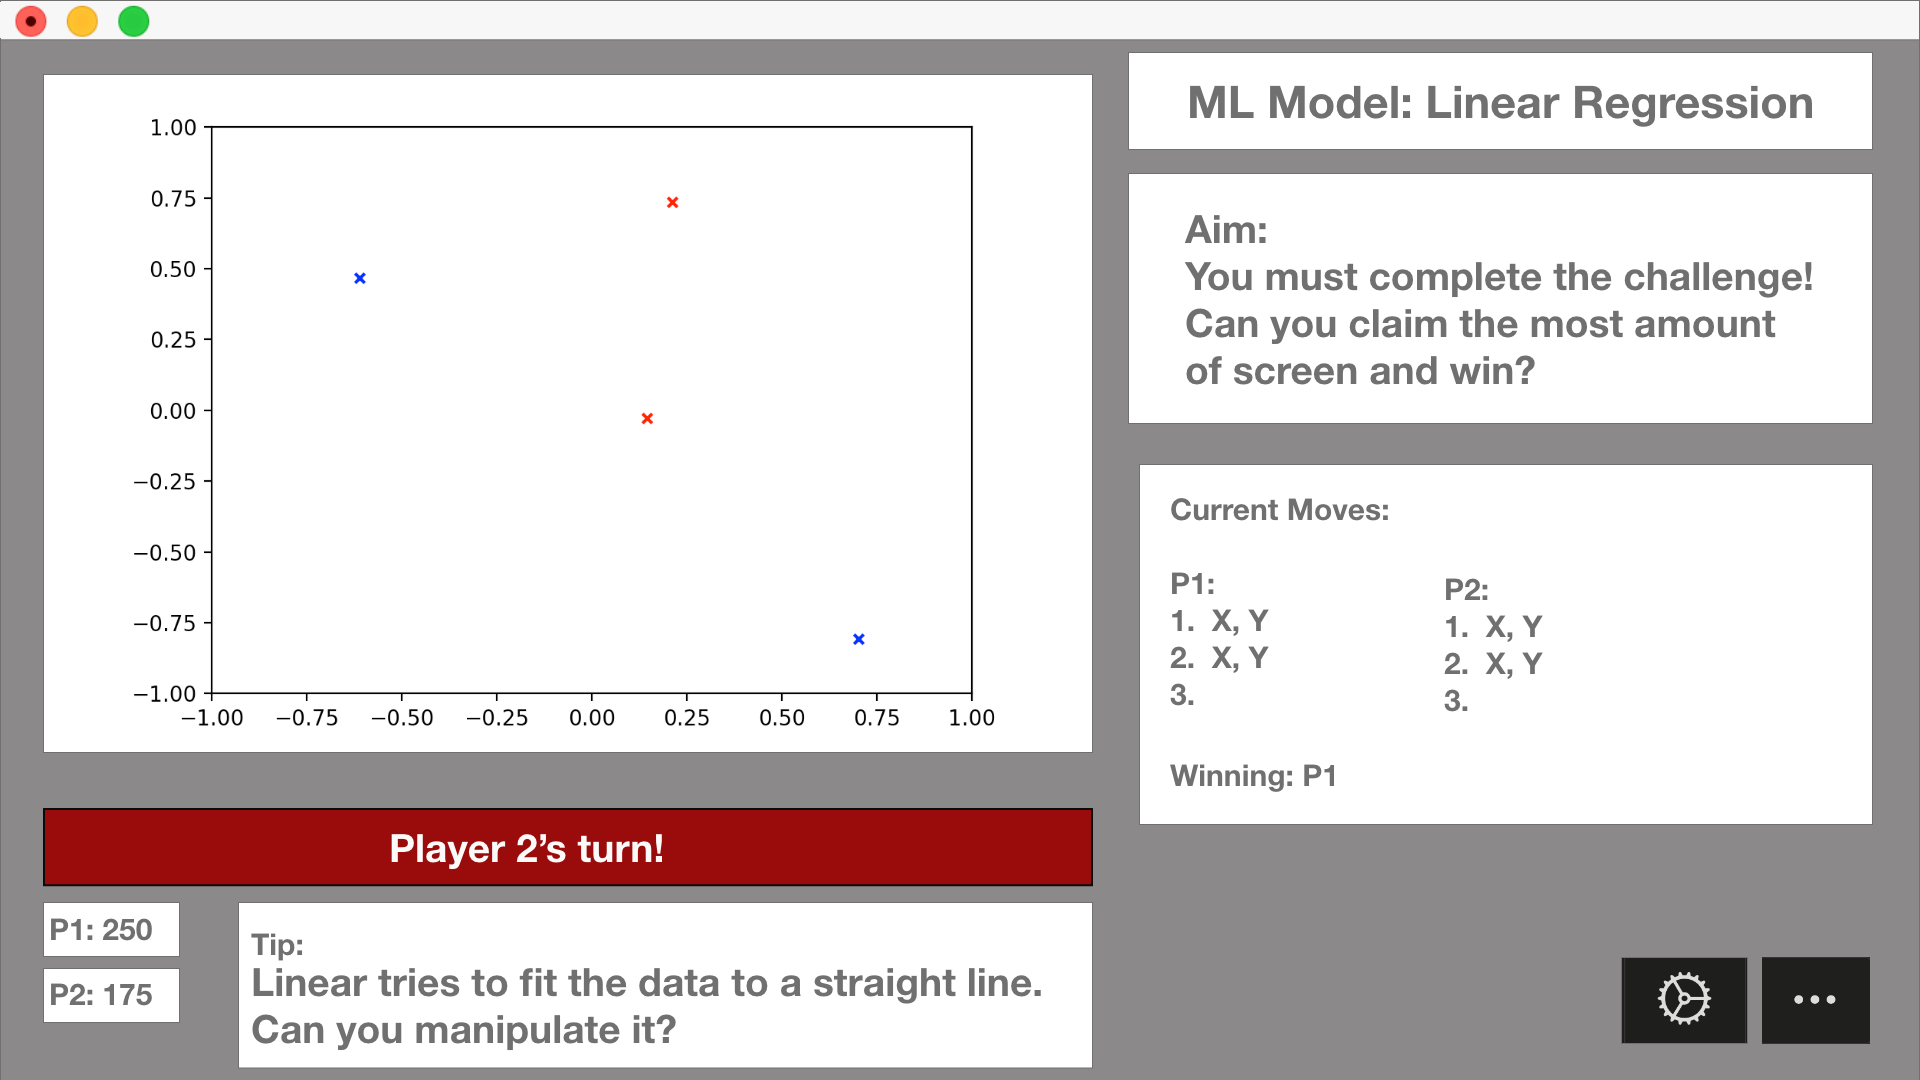
\includegraphics[width=12cm]{Web19203.png}
	\item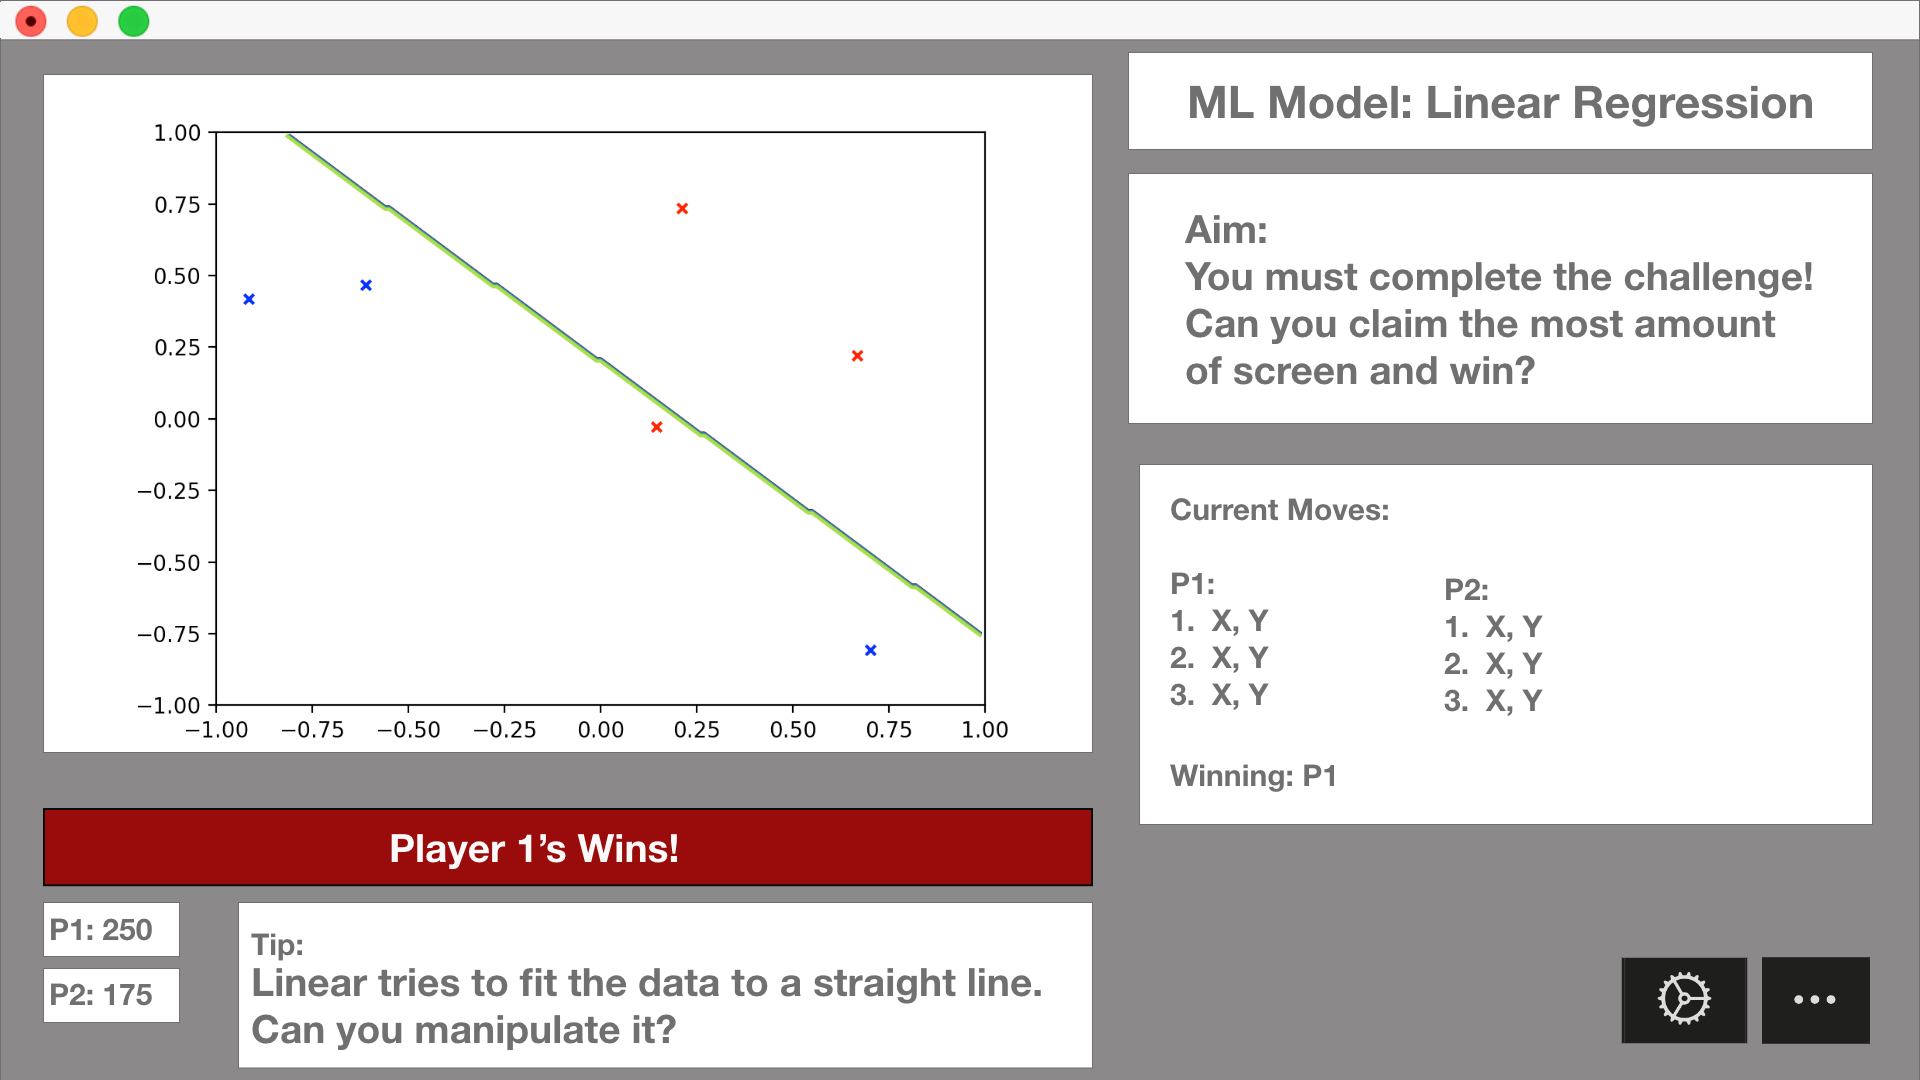
\includegraphics[width=12cm]{Web19204.png}
\end{center}

\section{Proposed Implementation Approach}
\subsection{Tools}
We plan to make the game using Python 3 \cite{reference here}. We plan to use this language due to the vast amount of packages and libraries available. Python has a vast amount of support within the Data Science and Machine Learning community, and it also has packages available to allow the create games and web applications. 

Visual Studio Code (VS Code) will be the chief text editor for implementing the game. Due to the nature of text editor, it will allow us to use all the Python libraries as well as any of the iPython notebook files. iPython notebooks are the primary file type for Jupyter Notebooks whereas VS Code allows user to edit multiple programming languages, which include Python and Jupyter Notebooks, in one place. However, with it being a text editor, it does lack the more advanced features we would expect in an IDE, but these are features we do not need.  

Jupyter Notebooks allows the code to be split up into cells, allowing us to be able to test out segments of code, without having to run all of the code in the file, which can be very helpful when trying to develop and implement some modularity features within the application.

We will be using Trello for the kanban tools. "Kanban" is the Japanese word for "visual signal" \cite{kanbanmeaning}. Using Kanban boards allows us to keep our work visible, this is to allow others to see what it is we are doing, and what is needed to get done. These will allow everyone to see the full picture and keep everyone on the same page.

David Anderson discovered that kanban boards get split into five components: Visual signals, columns, work-in-progress limits, a commitment point, and a delivery point \cite{anderson2010kanban}.

Kanban teams write all their project's work items onto cards, and these are usually one per card. The kanban board gets split into columns, with each column representing an activity which composes the workflow. All the cards change between the workflow until the activity is complete. The column workflow titles can be as simple as to do, in progress and completed. However, David suggests that there should be a work in progress (WIP) limit \cite{anderson2010kanban}. When a column has reached the limit, of three cards, all team members get expected to focus on the cards in progress. The WIP limits are critical for exposing bottlenecks in the workflow and maximizing flow. WIP limits give an early warning sign that too much work commissioned. Backlogs of ideas are where the ideas of the team and the customers get placed. The moment an idea gets picked up by a team member and work begins, this gets referred to as the commitment point \cite{anderson2010kanban}. When the product is finished and is ready for deployment, this stage gets referred to as the delivery point. The overall aim of the kanban is to take a card from the commitment point to delivery point as quick as possible.  

\subsection{Python Libraries} %subsubsubsection
The Python libraries that we will be using are Pygame for game development. [Add a brief description of it here]. This package will be the main one for creating the game's interface and game logic. 

For the main implemented machine learning algorithms that are within the game, a package called Scikit-learn will get used. [Add a brief description of it here]. This package will allow us to implement the algorithms [list them here] using the Python language.

\subsection{Development}
\subsubsection{Deployment Format}
The main application will be a desktop application.  Due to the potential size and scope of the application, the initial aim will be on creating a sleek and smooth learning game and tool, to get the understanding of machine learning across. However, due to the nature of the world at current, with more and more getting done online, a web application version of the application would be feasible. However, this can only be considered when the main application is completed to the expected level, with the desired user experience. Frameworks that would allow us to achieve this would be Python's web library called 'Django'.

\subsubsection{Developement style}
We will aim to create the app in a modular manner. By creating the application in a modular way, will allow us to create different aspects of the application at the same time. It is allowing us not to be limited to potential bottlenecks in development if particular modules are providing more issues than anticipated. We will then be intending for the Pygame user interface (UI) to be the factor that brings it all together, enabling all the different modules to be triggered based on the requirements of the game during the gameplay.\\
 \\
\textbf{Module Content}\\
As we will be developing the application modular, we will aim to have a module that will handle the educational content. This module will include the videos and explanations of the algorithms.

Another modular section will for each machine learning model. Each model being implemented and kept within its module section. Keeping them in their module will allow scalability to happen more pragmatically. Making sure that if an ML model is having issues while being implemented within the game, then it can be left out and not impact the overall performance or code base.

Then we aim to have another module that will focus on the interface and UI of the main game and any menu screens. We will aim to have the gamification aspects within an individual module as well.

\subsection{Proposed Evaluation Method of the Project}
In order to gain an understanding of how effective ou solution is, we will be carrying out several key testing strategies. These strategies include gameplay testing, unit testing, systems testing and finally, user test to gain insightful feedback from the target audience.

\section{Proposed Project Management}
Project management is crucial for any task that is about to get carried out, even more so the case for software development. As a famous Benjamin Franklin quote says "Failing to plan is planning to fail" \cite{plan_to_fail}. With this in mind, we must decide on the right project planning method that compliments our initial software design. From the waterfall method to Rapid application development (RAD) or the more modern methods of agile development, there are many methods that we could choose. We will explain the different methods that we could use and what ones would be best for our solution and intended development method.

\subsection{Proposed Life Cycle}
The profession of the software developer has existed since the first computers, but the practices and methods for developing software have evolved over timer \cite{SDLC}. The approaches have developed over the years to adapt to the ever-changing landscape of software development. The methods, known as software development life cycles (SDLC), vary in approach but fundamentally share the same goal. The main aims of the SDLC are to brake the development up into stage. However, what changes with different SDLC is how these stages get carried out. The different stages are planning, requirements, designing and prototyping, software development, testing, deployment, operations and maintenance \cite{SDLC}.

The first stage, planning, involves resource allocation, capacity planning, project scheduling, cost estimation and provisioning \cite{SDLC}. The primary outcome of this stage is to have an overall plan of what it is we have and what we will need to complete our goal within the constraints like costs and times allowed. The second stage, requirements, is where Subject Matter Experts (SMEs.) guide on what would be needed to carry out the stakeholders' requirements \cite{SDLC}. The third stage, design and prototyping, is where the software architects and developers begin to design the software. The outcome of this stage would be documentation on the intended design patterns and design wireframes of the intended final software. The fourth stage, development, is where the software starts to get made based on the decisions made in design and prototyping, following the chosen methodology. The outcome will be testable, tangible software. The fifth stage, testing, is considered the most crucial stage \cite{SDLC}. At this stage, it is essential to do all the code quality checking, unit testing, integration testing, performance testing and security testing. The sixth but by no mean final stage is deployment. This stage is when the code is ready to be shipped to the client or uploaded to the required app stores. However, the final stage is operations and maintenance. This stage is about making sure that the software is getting used how it should and that any bugs that did not initially get picked up in testing are correct and removed from the software. 

\subsubsection{Waterfall Method}
The waterfall method is a model where each section needs to get completed before we can move onto the next stage, like a waterfall flowing down. For example, before we can start analysing the requirements, we need to complete the planning stage. Following the seven critical stages of SDLC, one after each other.

Like all models, they have their advantages and disadvantages. Advantages that this model has is that it is easy to use and follow, and by the way it is all set up, every stage will get finished before the next stage starts. The waterfall method also allows for the project to be easily managed, resulting in easier documentation \cite{cscm01slidesl5}. However, some of the disadvantages are that it is not very useful if the requirements are not very clear at the beginning. Another disadvantage is that once we have moved to the next stage, it is tough to go back to a previous stage to make any changes which therefore creates higher risks to development and has less flexibility \cite{cscm01slidesl5}. The model is best when changes in the project are stable, and the project is small, with the project requirements are clearly defined.

\subsubsection{RAD: Rapid Application Development}
The overall aim of RAD is to create software projects with higher quality and faster by gathering requirements through workshops or focus groups. Then prototyping the product and then using reiterative user testing of designs early. RAD is the best model to use when we need something created quickly and have a pool of users available to test prototypes. However, this approach can be costly\cite{cscm01slides}. 

\subsubsection{Spiral Method}
The Spiral Model is an SDLC methodology that aids in choosing the optimal process model. It combines aspects of the incremental build model, waterfall model and prototyping model, but is different by a set of six invariant characteristics \cite{spiralmodel}. The Spiral Model main focus is on risk awareness and management. The risk-driven approach of the spiral model ensures the team is highly flexible within its approach, but also highly aware of the challenges they can expect down the road. The spiral model shines when stakes are highest, and significant setbacks are not an option \cite{spiralmodel}.


\subsubsection{Agile Development}
The Agile methodology is a process by which a team can manage a project, which gets achieved by breaking up the project into several stages. It required constant collaboration with stakeholders which leads to continuous iterations of improvement. In essence, Agile development is not a set methodology more of a manifesto that is aiming to uncover better ways to develop software. "Individuals and interactions over processes and tools. Working software over comprehensive documentation. Customer collaboration over contract negotiation. Responding to change over following a plan \cite{agilemanifesto}."

\subsubsection{Decided Method}
The project's requirements have features that lend themselves well to the waterfall methodology. However, we would like to have an element of agile methodology within the development due to the application intending to get created in a modular way. By using the waterfall method it will allow us to have a clear plan and requirements of what is needed, but by using the agile method, we can then rotate between the software development and testing stage.




\begin{landscape}
\subsection{Gantt chart}
	\begin{center}
		\item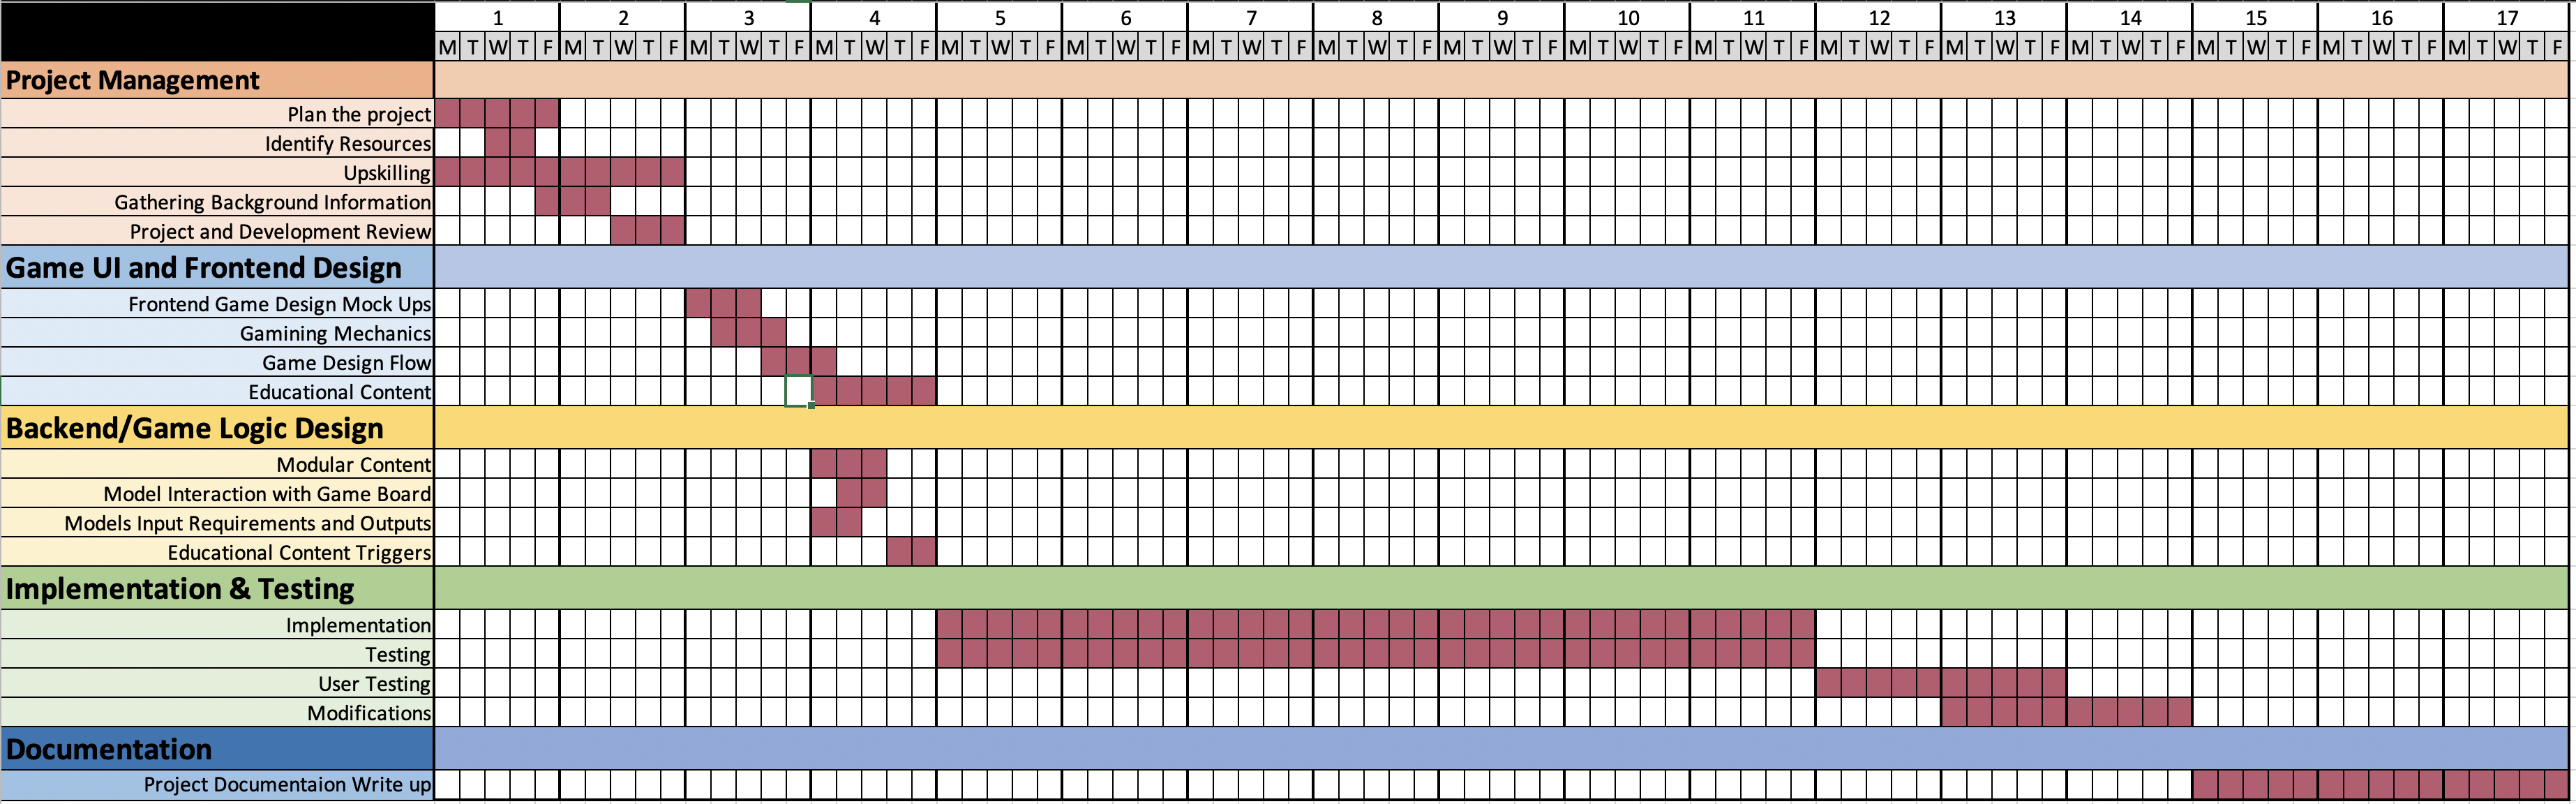
\includegraphics[width=27cm]{ganttchart.png}
	\end{center}
\end{landscape}


\subsection{Risk management}
\begin{center}
	\item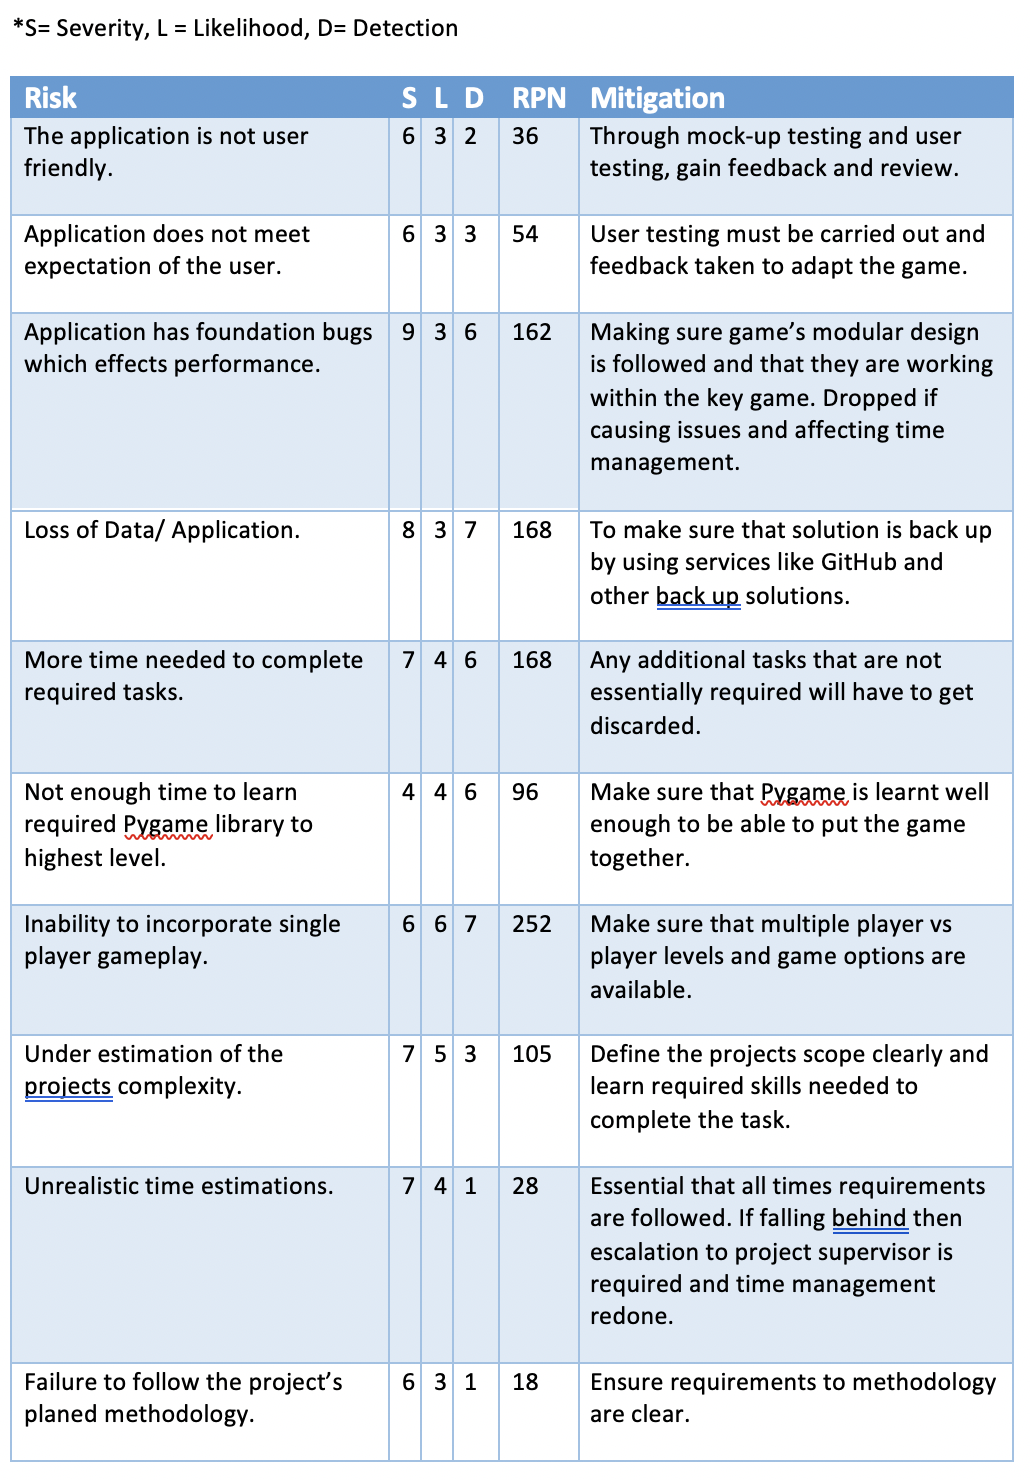
\includegraphics[width=13cm]{riskman.png}
\end{center}

\section{Summary}



This project is probably more Waterfall than any project I've had before. Remember to compare to others and give a justified choice.

%\medskip
\newpage
%\begin{appendices}
%	\section{Total count for Country}
%	\label{appendix:totalcountall}
%	%% Add image of graph here.
%	%\includegraphics[scale=0.5]{totalcount}
%	
%	\section{Lift Table of Items Whole Dataset}
%	\label{appendix:wholelift}
%	%\includegraphics[scale=0.2]{wholelift}

%	\section{Confidence Table of Items Whole Dataset}
%	\label{appendix:wholeconf}
	%\includegraphics[scale=0.2]{wholeconf}
	
%	\section{Lift Table of United Kingdom Items}
%	\label{appendix:uklift}
	%% Add image of graph here.
	%\includegraphics[scale=0.2]{uklift}
	
%	\section{Confidence Table of United Kingdom Items}
%	\label{appendix:ukconf}
	%\includegraphics[scale=0.2]{ukconf}
	
%	\section{Lift Table of Germany Items}
%	\label{appendix:germanylift}
	%\includegraphics[scale=0.2]{germanylift}
	
%	\section{Confidence Table of Germany Items}
%	\label{appendix:germanyconf}
	%\includegraphics[scale=0.2]{germanyconf}
	
%	\section{Lift Table of France Items}
%	\label{appendix:francelift}
	%\includegraphics[scale=0.2]{francelift}
	
%	\section{Confidence Table of France Items}
%	\label{appendix:franceconf}
	%\includegraphics[scale=0.2]{franceconf}
	
%	\section{Lift Table of Erie Items}
%	\label{appendix:eirelift}
	%\includegraphics[scale=0.19]{eirelift}
	
%	\section{Confidence Table of Eire Items}
%	\label{appendix:eireconf}
	%\includegraphics[scale=0.19]{eireconf}
	
%\end{appendices}

%\newpage

%Sets the bibliography style to UNSRT and imports the 
%bibliography file "samples.bib".
\bibliographystyle{acm}

{\footnotesize
	\bibliography{samples}
}


\end{document}